\documentclass[a4paper, 10pt]{article}
\usepackage{amsmath}
\usepackage{amssymb}
\usepackage[justification=raggedright,singlelinecheck=false]{caption}
\usepackage[top=1in, bottom=1in, left=1.25in, right=1in]{geometry}
\usepackage{graphicx}
\usepackage{float}
\usepackage{multirow}
\usepackage[table]{xcolor}
\usepackage{hyperref}
\usepackage{subcaption}
\usepackage{tabularx}

\title{Gaussian Processes for Time Series}
\date{\today}
\author{Raphaela Azar and Sbonelo Gumede \\
Supervised by Prof. Birgit Erni\\
The University of Cape Town}

\begin{document}

   \maketitle

   \begin{flushleft}

   \section*{Introduction}

   In this paper we hope to define what is a Gaussian process. How can you use a Gaussian process for time series analysis? Compare the peformance of a Gaussian process to other time series analysis models such as state-space models. An area of application included is predicting the level of air pollution in the Table View station in Cape Town for the year of 2019. Another area of application is predicting the gold price for South Africa for the year of 2020. This is done in a Bayesian framework in order to make probabilistic statements and obtain a predictive distribution for future forecasts.

   \vspace{1em}

   A Gaussian process is a stochastic process denoted by $\{X_{t} \}_{t \in \mathcal{I}}$, where the parameter space $\mathcal{I}$ and the state space $\mathcal{U}$ are real numbers. 
   At each point $t \in \mathcal{I}$, the state $X_{t} \sim \mathcal{N}(f(x_{t}), \, g(x_{t}, \, x_{t}))$, where $f(x_{t})$ is a mean function and $g(x_{t}, \, x_{t}) \geq 0$ is the covariance function.  
   Consider a simple example shown in figure 1, where $f(x_{t}) = x_{t} \, \text{and} \, g(x_{t}, \, x_{t}) = 1$.
   
   \begin{figure}[H]
      \centering
      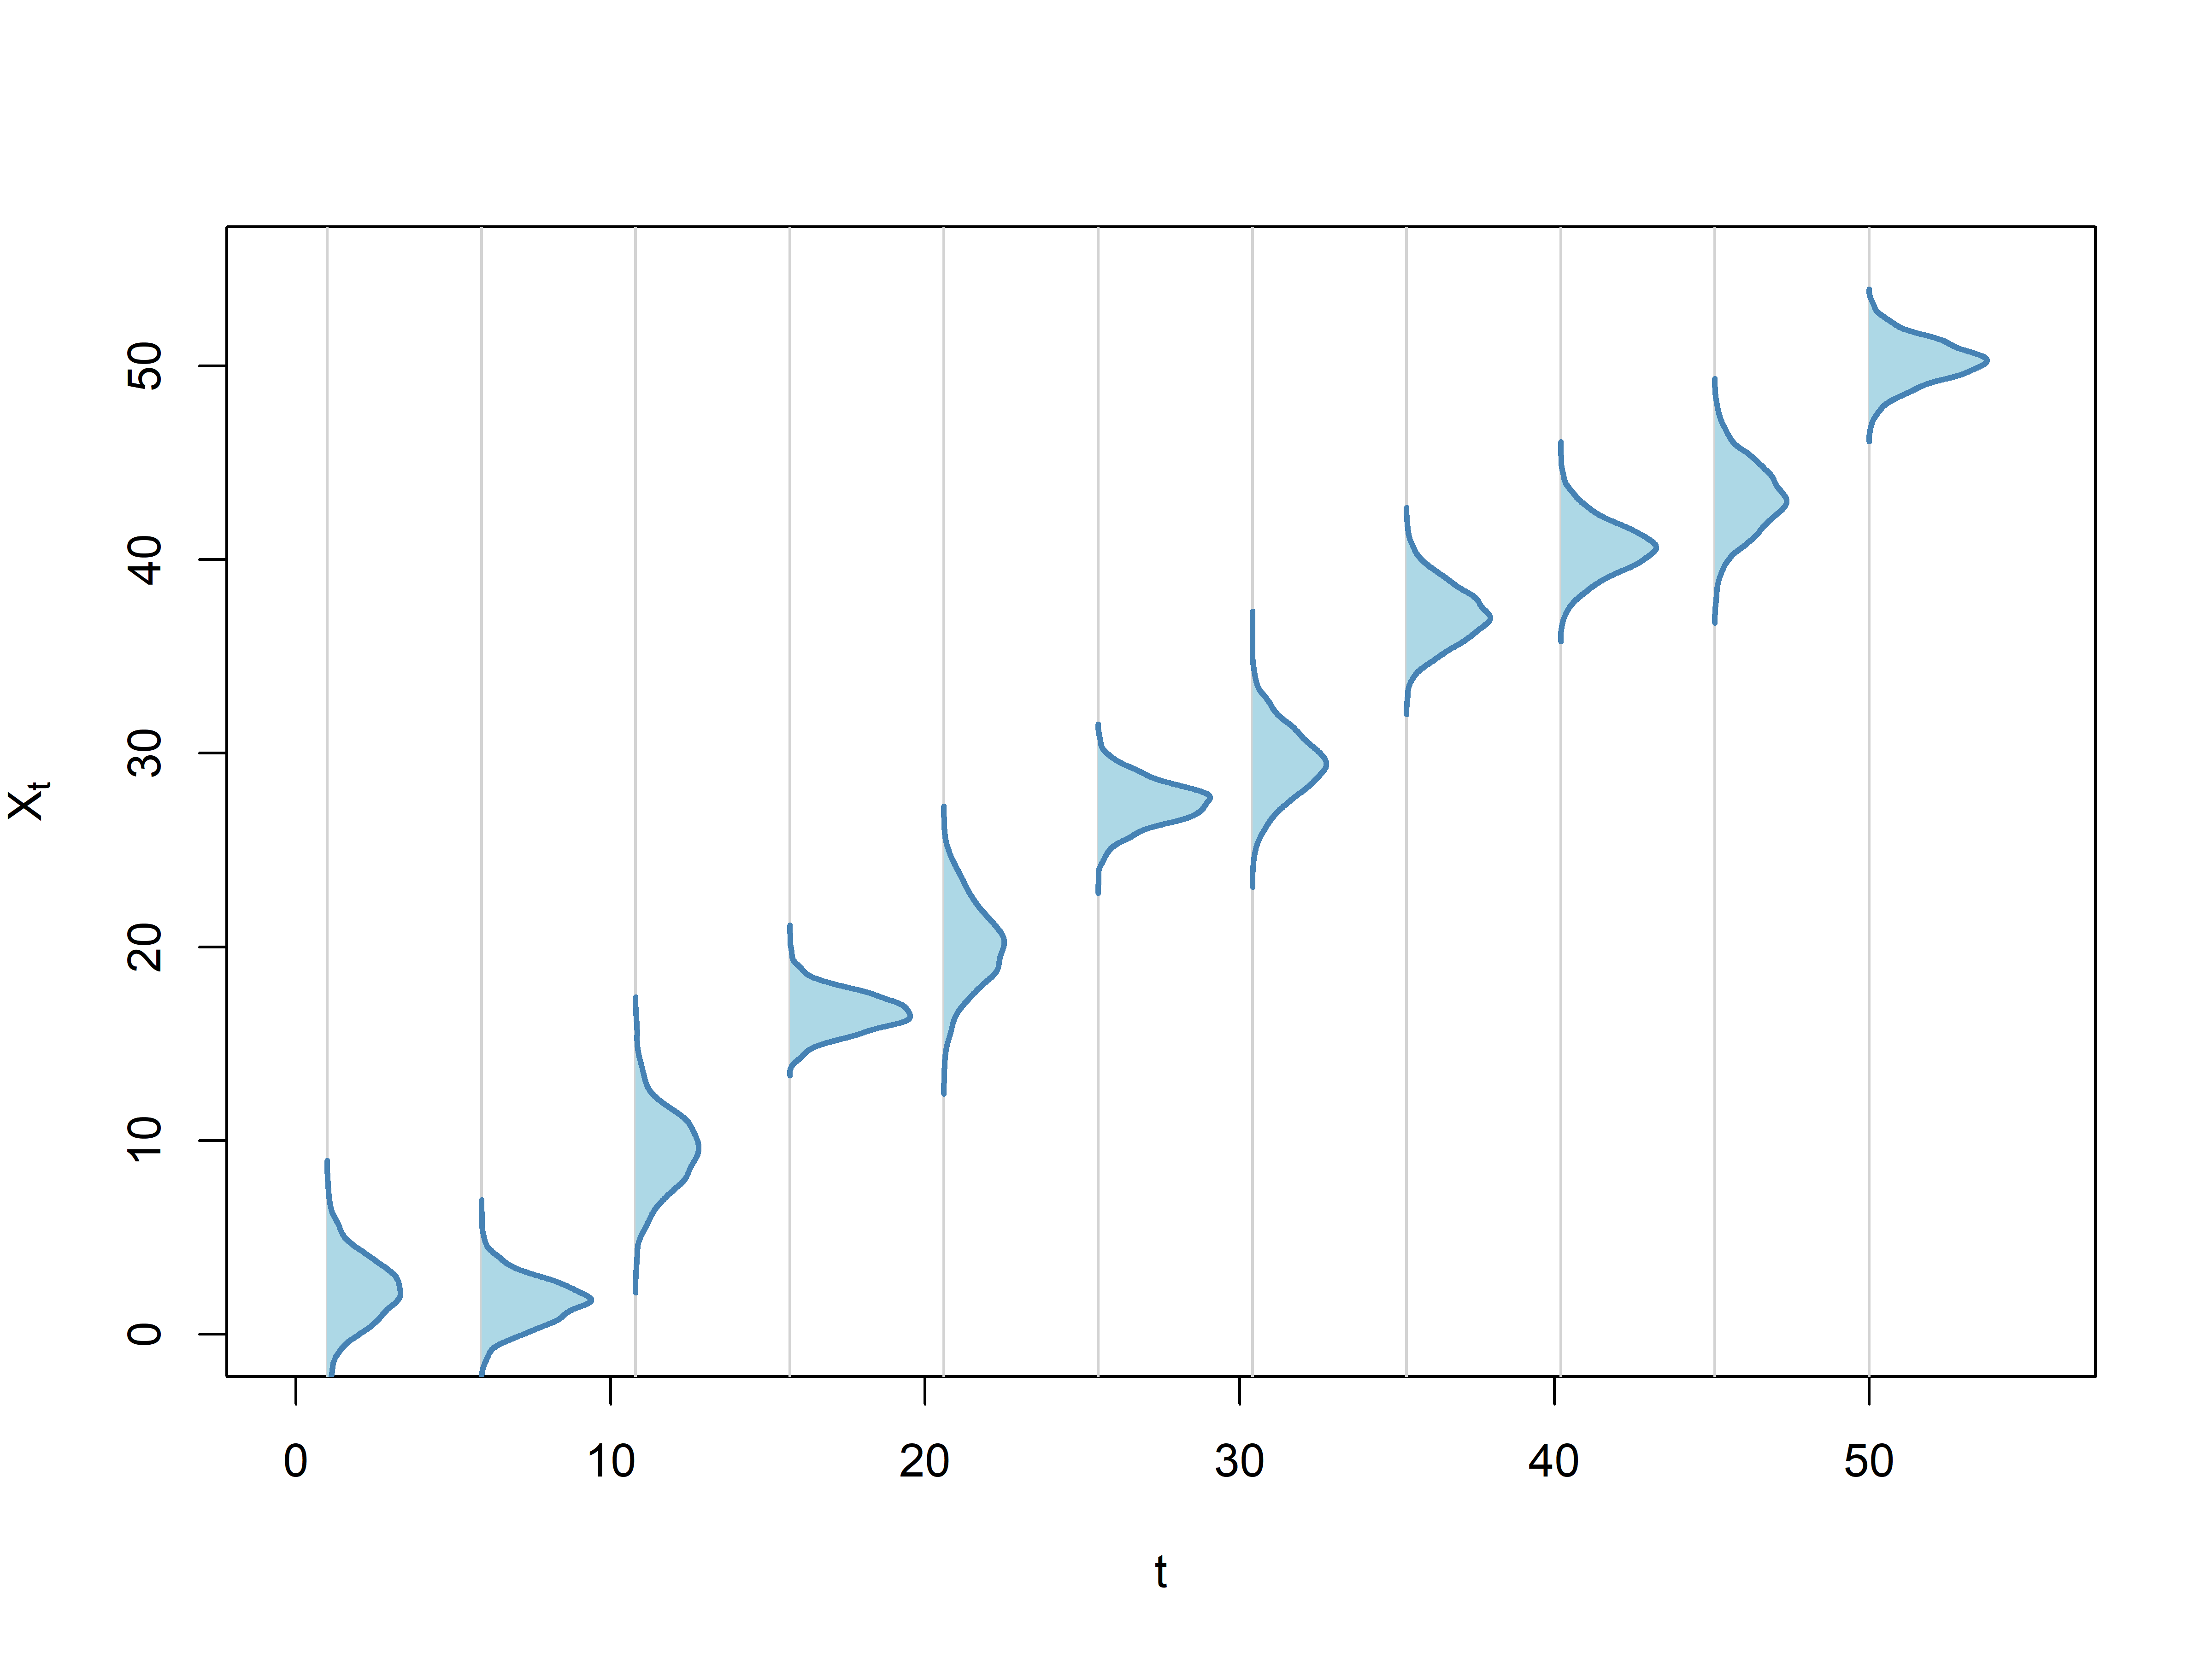
\includegraphics[width=0.48\linewidth]{../img/gp.png}
      \caption{\textit{An example of a Gaussian process on $\{0, 10, \ldots, 50\}$.}}
   \end{figure}
   
   A special property of Gaussian processes is that if you take a countable finite set of random variables $\{X_{1}, \, \ldots, \, X_{p}\}$ their joint distribution is 
   $
   \mathbf{X} =
   \begin{bmatrix}
      X_{1} \\
      \vdots \\
      X_{p}
   \end{bmatrix}
   \:
   \sim \mathcal{N}_{p}(\boldsymbol{\mu}, \, \boldsymbol{\Sigma}),
   \:
   \text{where}
   \:
   \boldsymbol{\mu} = 
   \begin{bmatrix}
      f(x_{1}) \\
      f(x_{2}) \\
      \vdots \\
      f(x_{p})
   \end{bmatrix}  
   \: 
   \text{and}
   \:
   \boldsymbol{\Sigma} = 
   \begin{bmatrix}
      g(x_{1}, \, x_{1}) & g(x_{1}, \, x_{2}) & \cdots & g(x_{1}, \, x_{p}) \\
      g(x_{2}, \, x_{1}) & g(x_{2}, \, x_{2}) & \cdots & g(x_{2}, \, x_{p}) \\
      \vdots & \vdots & \ddots & \vdots \\
      g(x_{p}, \, x_{1}) & g(x_{p}, \, x_{2}) & \cdots & g(x_{p}, \, x_{p})
   \end{bmatrix}$.

   \vspace{1em}
   
   Often in the literature people use $f(x_{t}) = 0$ and $g(x_{i}, \, x_{j}) = \alpha^{2} \text{exp}(- \frac{1}{2} (\frac{|x_i - x_j|}{\rho})^2) + \sigma\delta_{ij} \, \text{where}, \, \delta_{ij} = 1 \, \text{for} \, i=j \, \text{and} \, \delta_{ij} = 0 \, \text{for} \, i \neq j$, $\alpha$, $\rho$, and $\sigma$ are hyperparameters. The latter is known as the squared-exponential kernel. Some kernel functions common in the literature are the following:

   \vspace{1em}
   
   There are two ways of modeling time series data. The first one is functional mapping $y = f(x) + e$, where $y$ is the response variable, $x$ is the explanatory variable, and $e$ is typically white additive noise. The noise is assumed to be uncorrelated with one another. Although the simplicity of functional mapping is attractive, functional mapping neglects the time component rendering it useless for our purposes. The second one is curve fitting, where $x$ is often time and $y$ is the response variable. This is ideal for our purposes since we are accounting for the time dependence between successive observations.

   \section*{Air pollution example}
   \subsection*{Exploratory data analysis}
   
      \begin{table}[H]
         \centering
         \begin{tabularx}{\textwidth}{|l|l|X|l|}
         \hline
         \text{Variable} & \text{Name} & \text{Description} & \text{Unit} \\
         \hline
         \(\text{NO}_{2}\) & Nitrogen dioxide & A harmful gas from vehicles and industry. & \(\mu\text{g}/\text{m}^{3}\) \\
         \(\text{PM}_{10}\) & Particulate matter 10 & Small inhalable dust particles. & \(\mu\text{g}/\text{m}^{3}\) \\
         \(\text{SO}_{2}\) & Sulphur dioxide & Mainly from burning fossil fuels. & \(\mu\text{g}/\text{m}^{3}\) \\
         Speed & Wind speed & How fast the wind is moving. & m/s \\
         \hline
         \end{tabularx}
         \caption{\textit{Description of variables of the air pollution dataset.}}
         \label{tab:variable_description}
      \end{table}

      \begin{table}[H]
         \centering
         \begin{tabularx}{\textwidth}{|l|X|X|X|X|X|X|X|X|}
            \hline
            Variable & Min. & 1st Qu. & Median & Mean & Std. & 3rd Qu. & Max. & NA's \\
            \hline
            NO$_2$   & 0.0 & 5.0  & 9.0  & 12.73 & 10.72 & 17.0 & 113.0 & 734 \\
            PM$_{10}$ & 0.0 & 12.0 & 17.0 & 19.82 & 12.30 & 24.0 & 158.0 & 298 \\
            SO$_2$   & 0.0 & 2.0  & 3.0  & 6.20  & 11.30 & 5.0  & 142.0 & 638 \\
            Speed    & 0.5 & 2.3  & 3.6  & 3.74  & 1.71  & 4.9  & 11.2  & 918 \\
            \hline
         \end{tabularx}
         \caption{\textit{Summary statistics of the air pollution dataset.}}
         \label{tab:summary_statistics}
      \end{table}

      \begin{figure}[H]
         \centering
         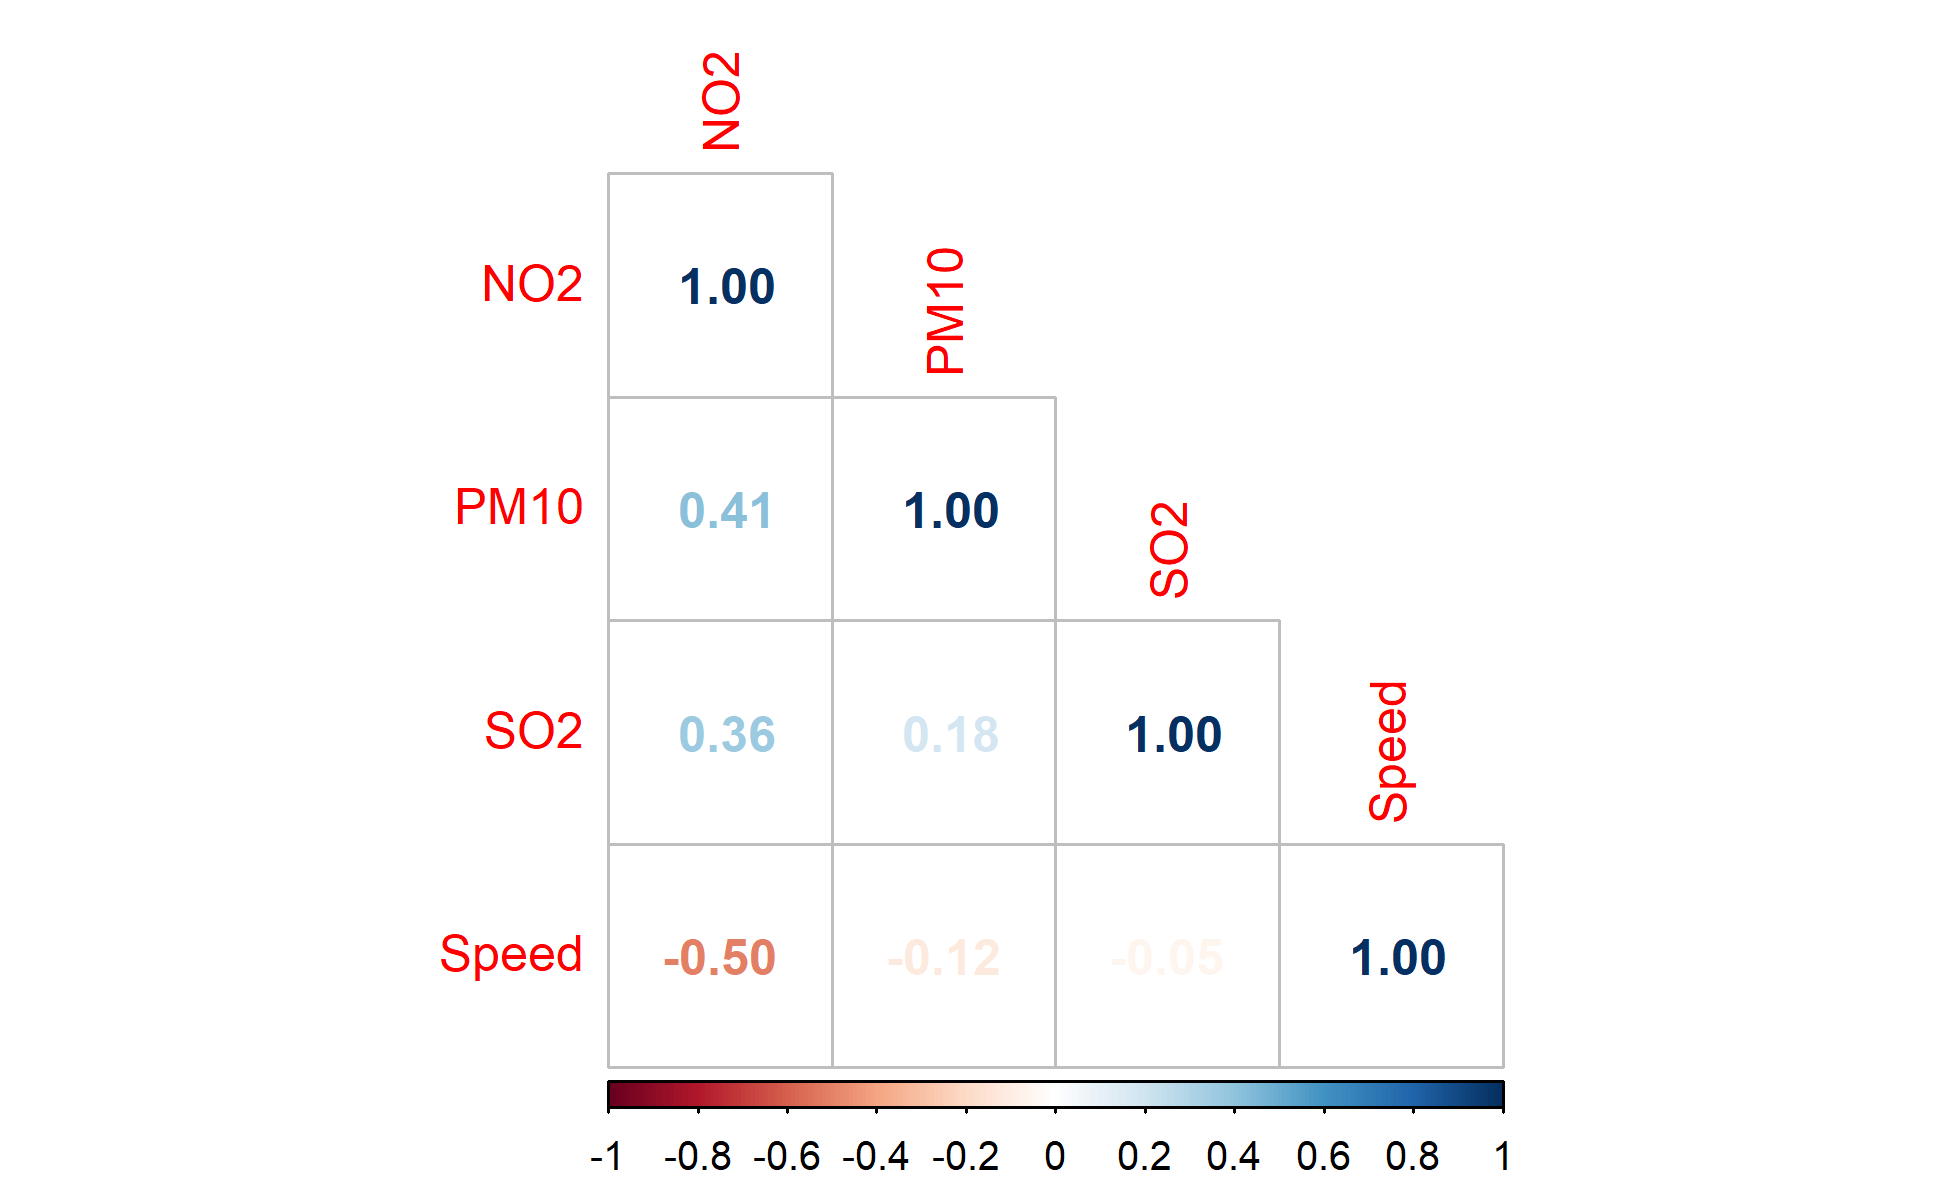
\includegraphics[width=0.48\linewidth]{../img/corrplot.png}
         \caption{\textit{Correlation plot of the air pollution dataset.}}
      \end{figure}

      Our response variable $\text{NO}_{2}$ appears to be moderately positively correlated with $\text{PM}_{10}$ and $\text{SO}_{2}$, and moderately negatively correlated with Speed. These are not ideal explanatory variables since we typically would like them to be strongly correlated with the response variable. The explanatory variables are weekly correlated with one another, whether it be positive or negative correlation. This is ideal since some models do not work well with correlated explanatory variables, often leading to unstable point estimates and inflated standard errors.

      \vspace{1em}

      Before looking at the data. The proposal mean function is $f(x_{t}) = x_{t}^{T} \beta + e$ and the proposal covariance function is $g(x_{i}, x_{j}) = \alpha^{2} \text{exp}(- \frac{1}{2} (\frac{|x_i - x_j|}{\rho})^2) + \sigma\delta_{ij} \, \text{for} \, i,j \in \mathcal{I}$. This allows us to capture the trend (if it exists) in the time series. This also allows us to capture the correlation structure of the data. The squared-exponential kernel is chosen because it is a natural way of describing the correlation decay.

      \vspace{1em}

      The prior distributions of the exponantiated quadratic kernel are the following: $\alpha \sim \text{half-normal}(0, 1)$, $\rho \sim \mathcal{IG}(20, 10)$, and $\sigma \sim \text{half-normal}(0, 1)$.

      \begin{figure}[H]
         \centering
         \begin{subfigure}{0.48\linewidth}
            \centering
            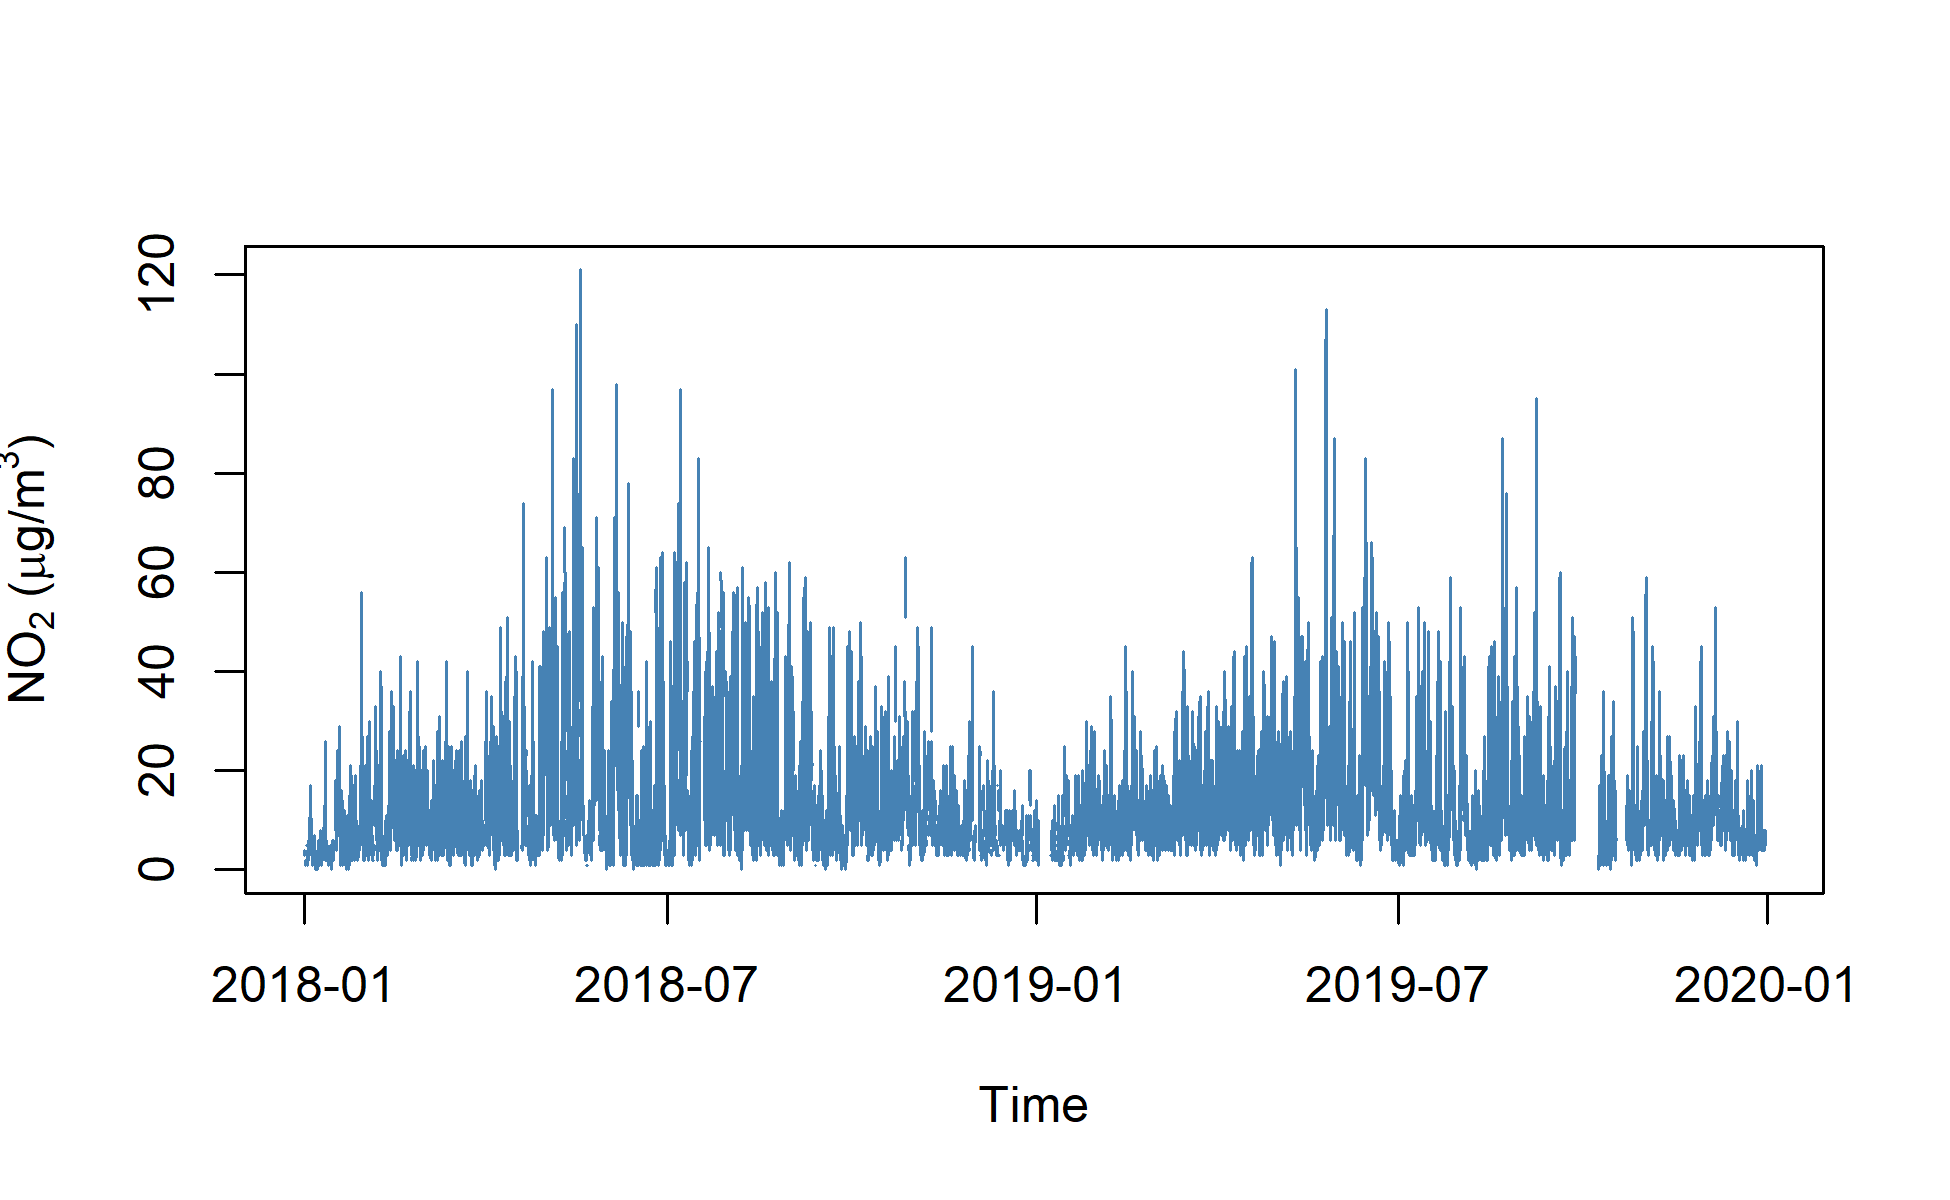
\includegraphics[width=\linewidth]{../img/extracted_no2.png}
         \caption{Nitrogen dioxide}
         \end{subfigure}
         \hfill
         \begin{subfigure}{0.48\linewidth}
            \centering
            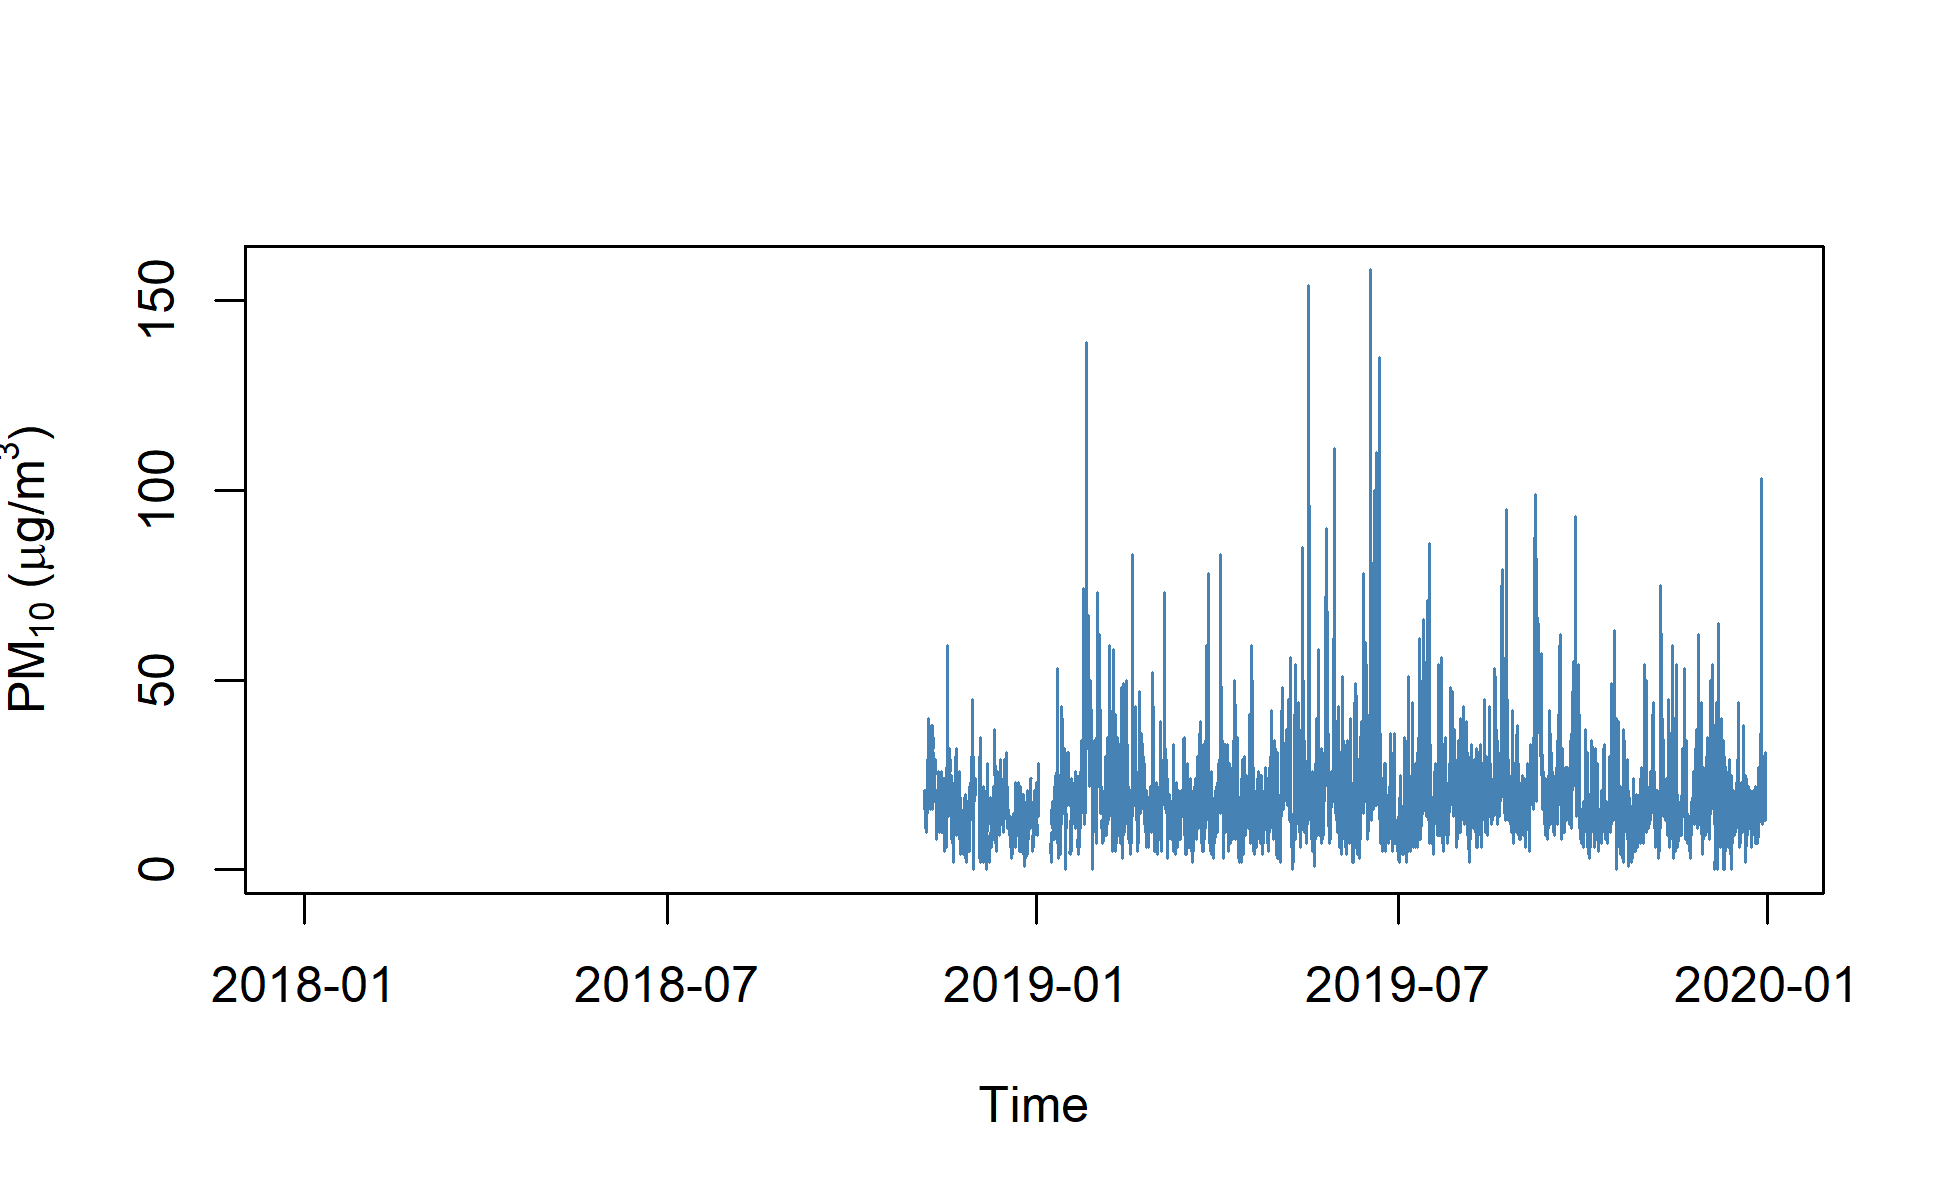
\includegraphics[width=\linewidth]{../img/extracted_pm10.png}
            \caption{Particulate matter 10}
         \end{subfigure}
         
         \vspace{0.5em}

         \begin{subfigure}{0.48\linewidth}
            \centering
            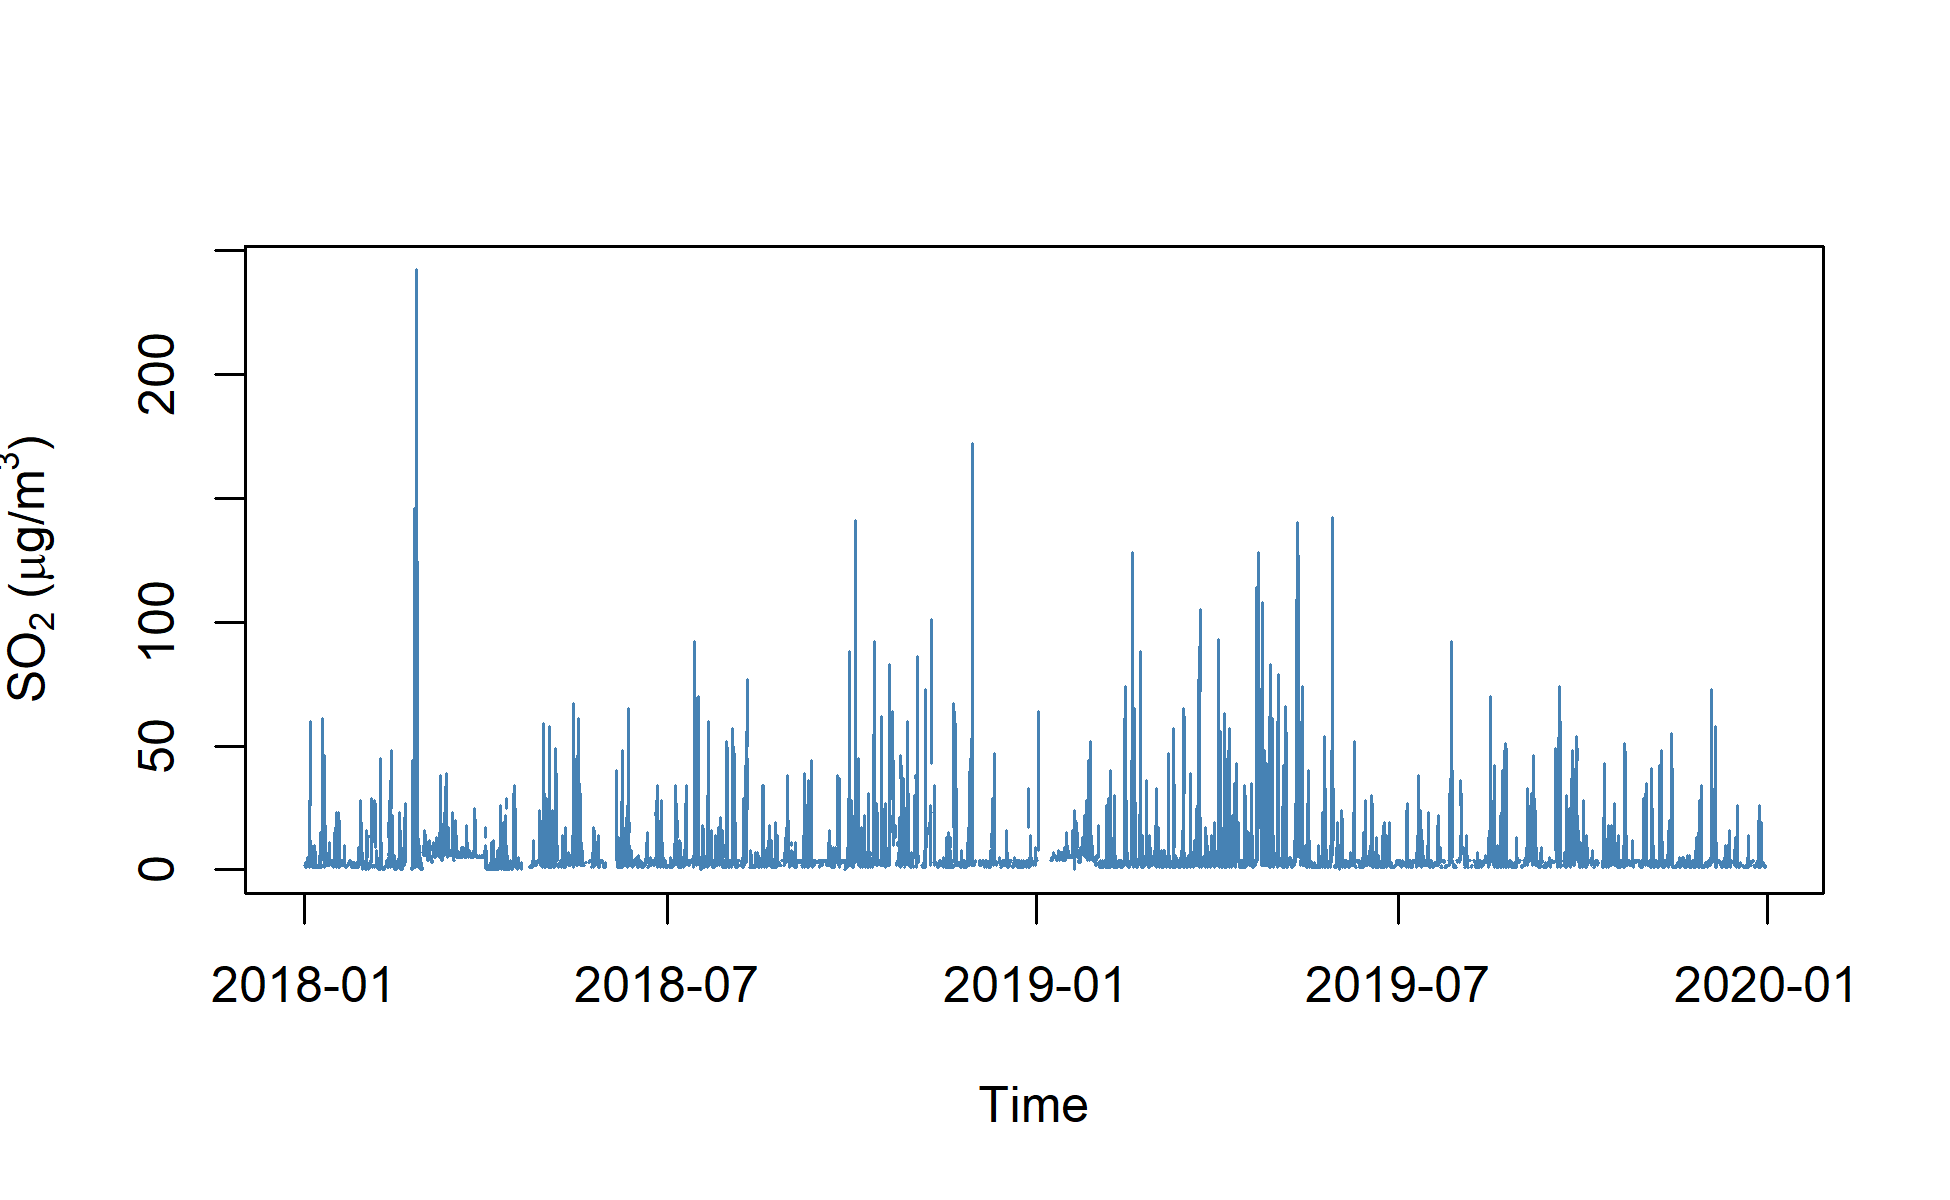
\includegraphics[width=\linewidth]{../img/extracted_so2.png}
         \caption{Sulphur dioxide}
         \end{subfigure}
         \hfill
         \begin{subfigure}{0.48\linewidth}
            \centering
            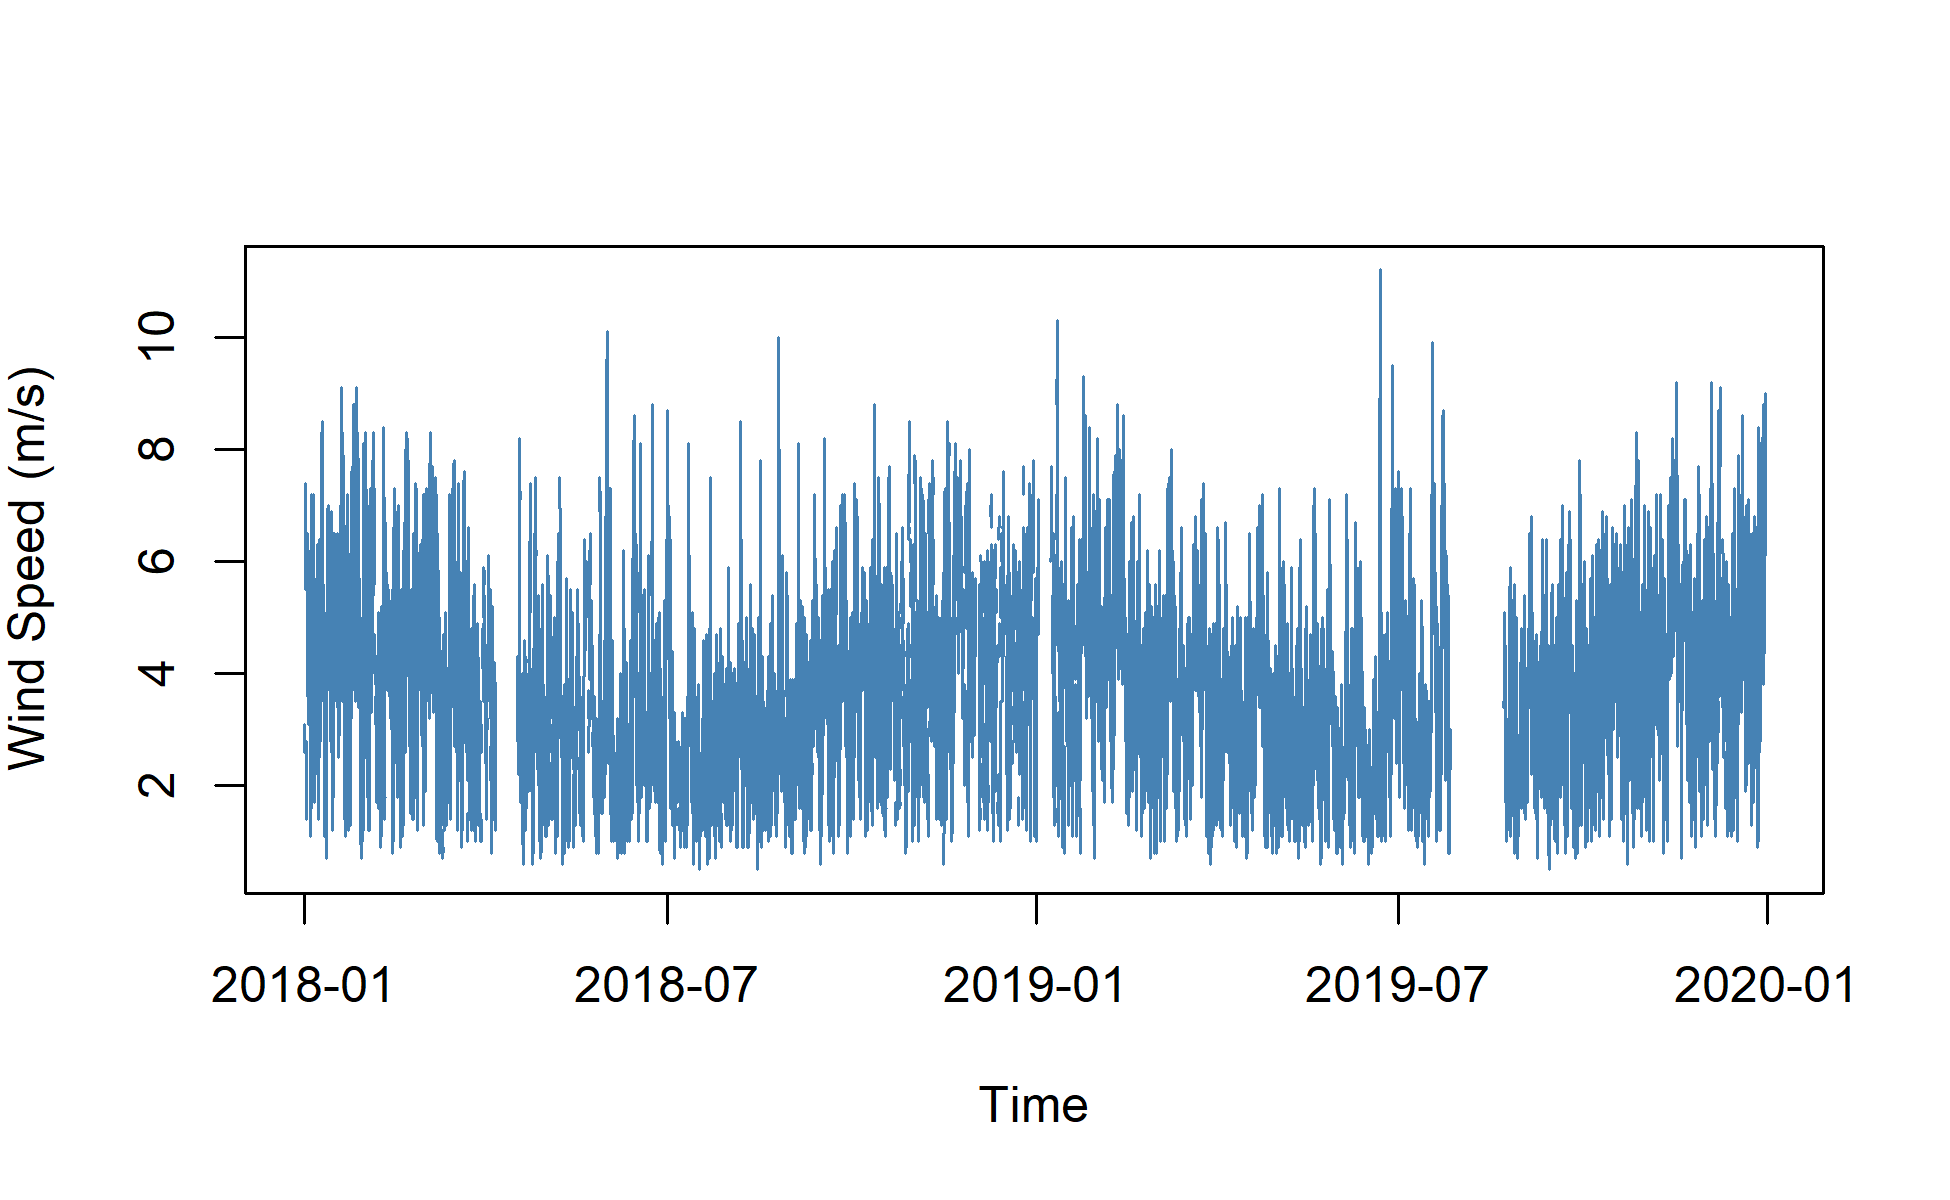
\includegraphics[width=\linewidth]{../img/extracted_speed.png}
            \caption{Wind speed}
         \end{subfigure}

         \caption{\textit{Time-series plots of nitrogen dioxide and mereorological processes from 01/01/2018 to 31/12/2019 measured hourly. Similar cyclic patterns can be observed in the meteorological processes, and a weaker seasonality component can be noted in the yearly nitrogen dioxide processes.}}
      \end{figure}

      \begin{figure}[H]
         \centering
         \begin{subfigure}{0.48\linewidth}
            \centering
            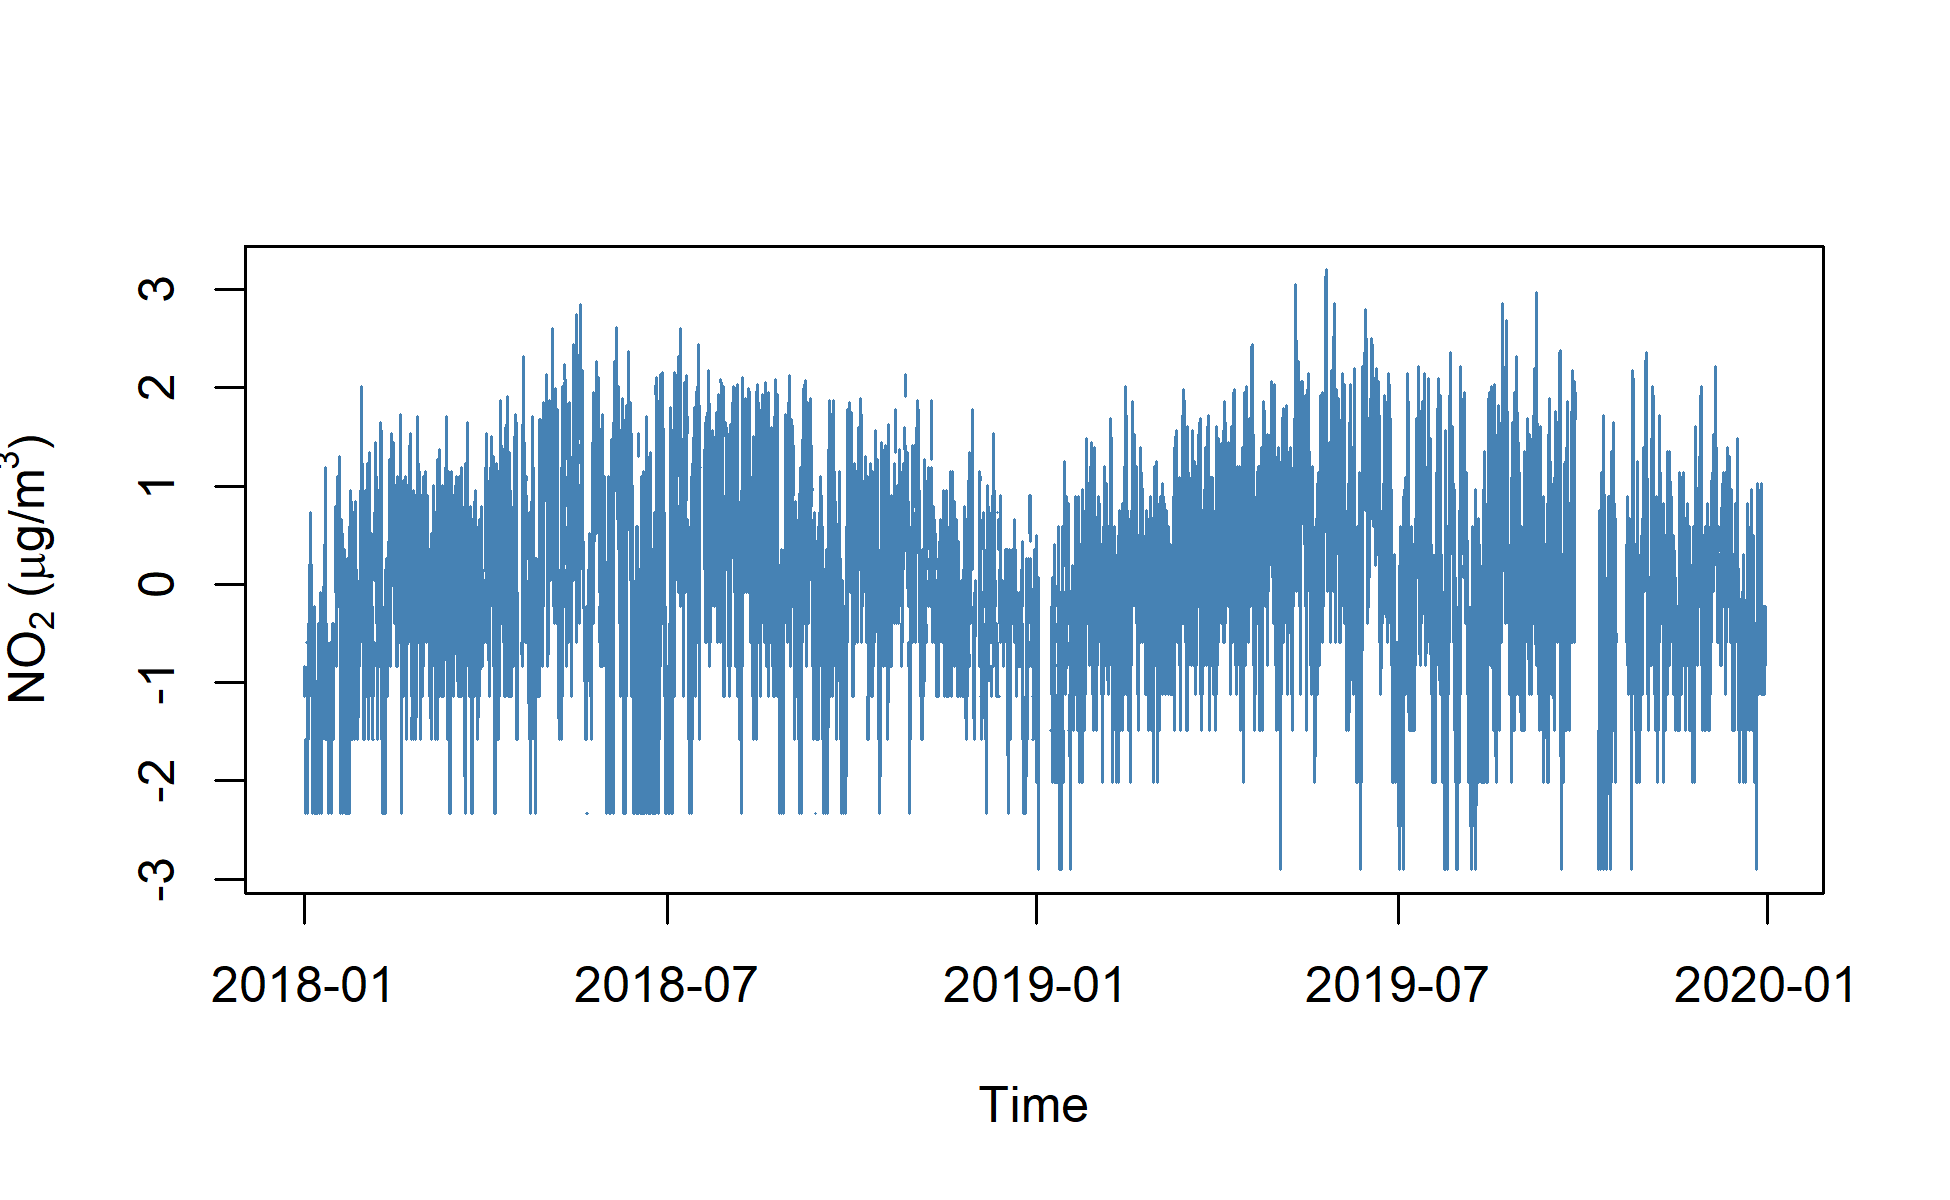
\includegraphics[width=\linewidth]{../img/transformed_no2.png}
         \caption{Nitrogen dioxide}
         \end{subfigure}
         \hfill
         \begin{subfigure}{0.48\linewidth}
            \centering
            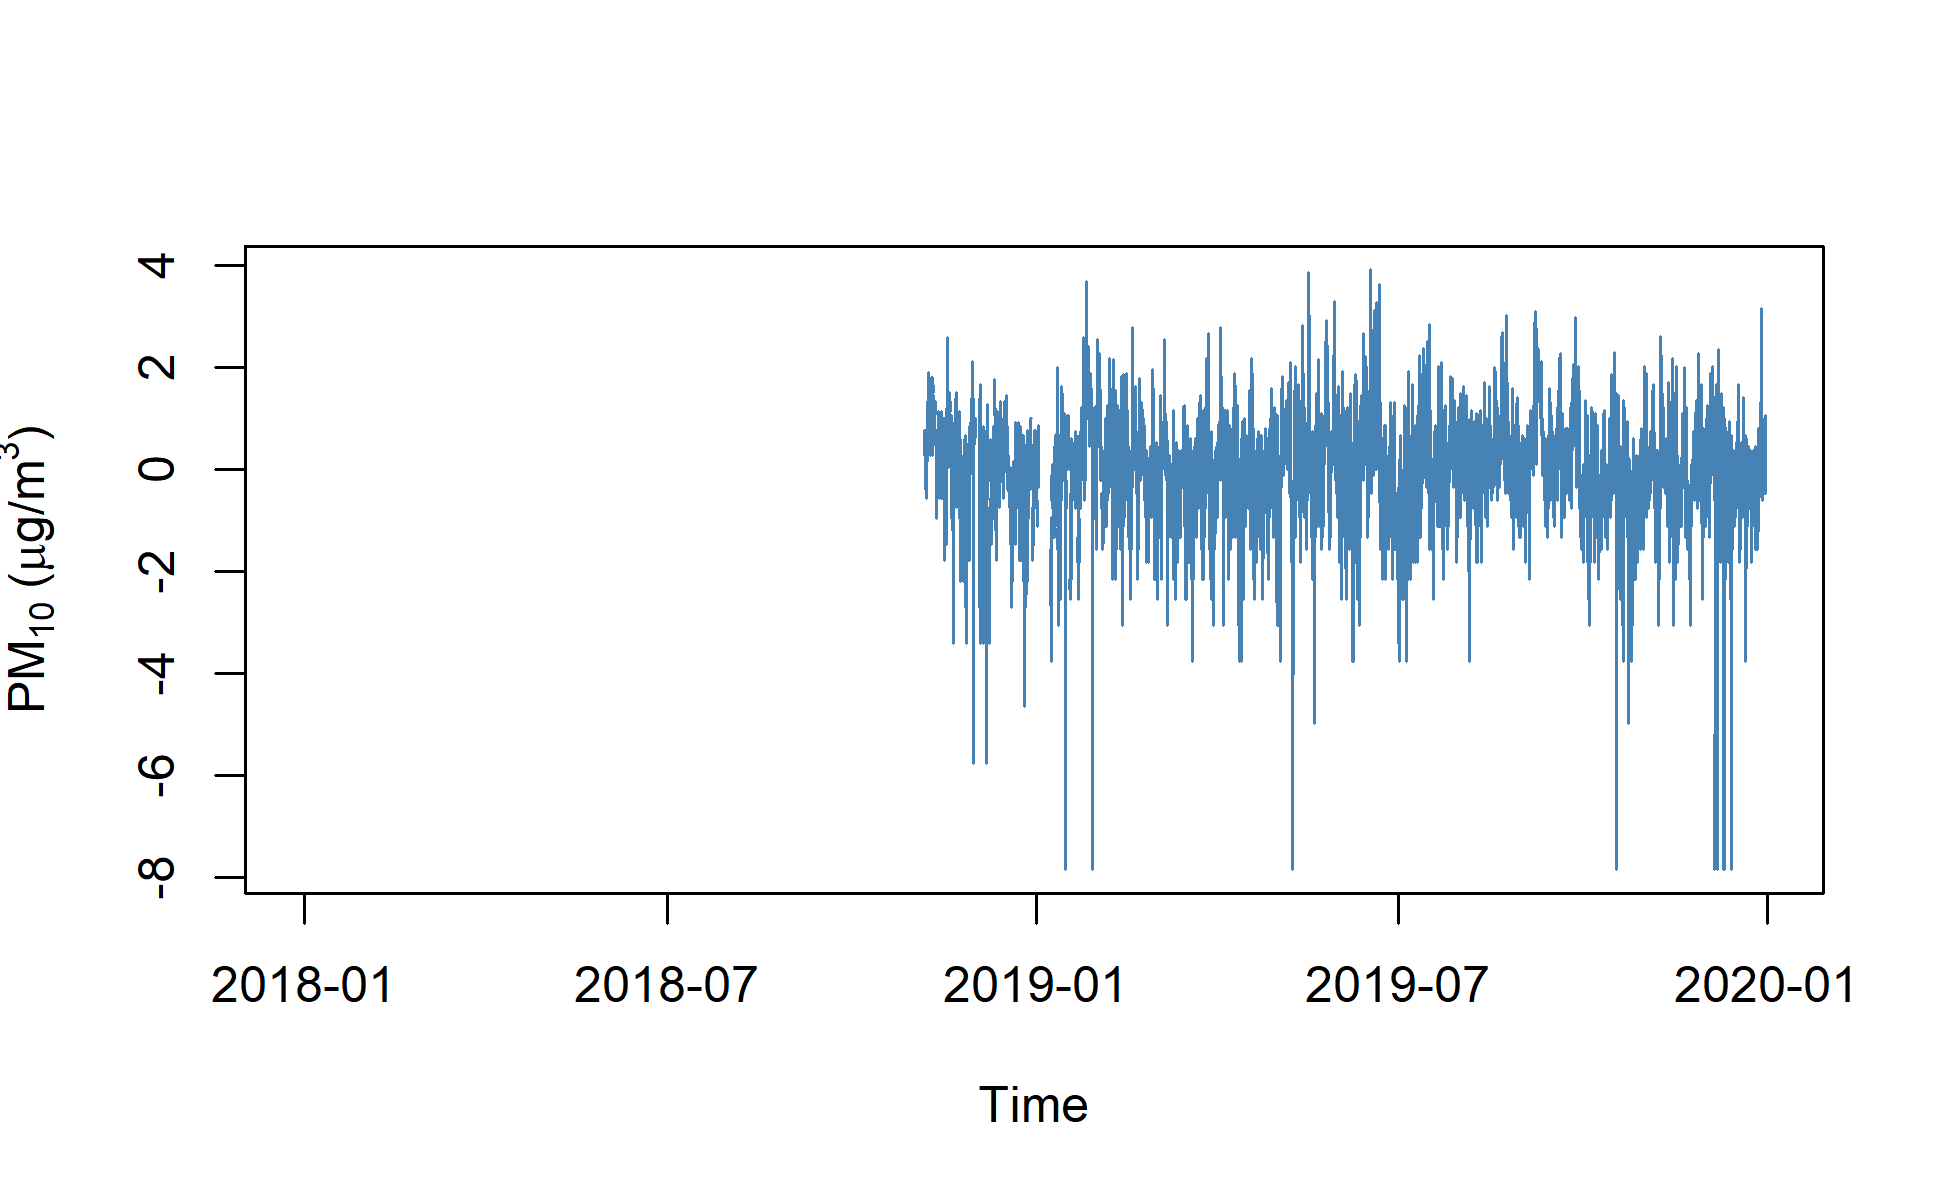
\includegraphics[width=\linewidth]{../img/transformed_pm10.png}
            \caption{Particulate matter 10}
         \end{subfigure}
         
         \vspace{0.5em}

         \begin{subfigure}{0.48\linewidth}
            \centering
            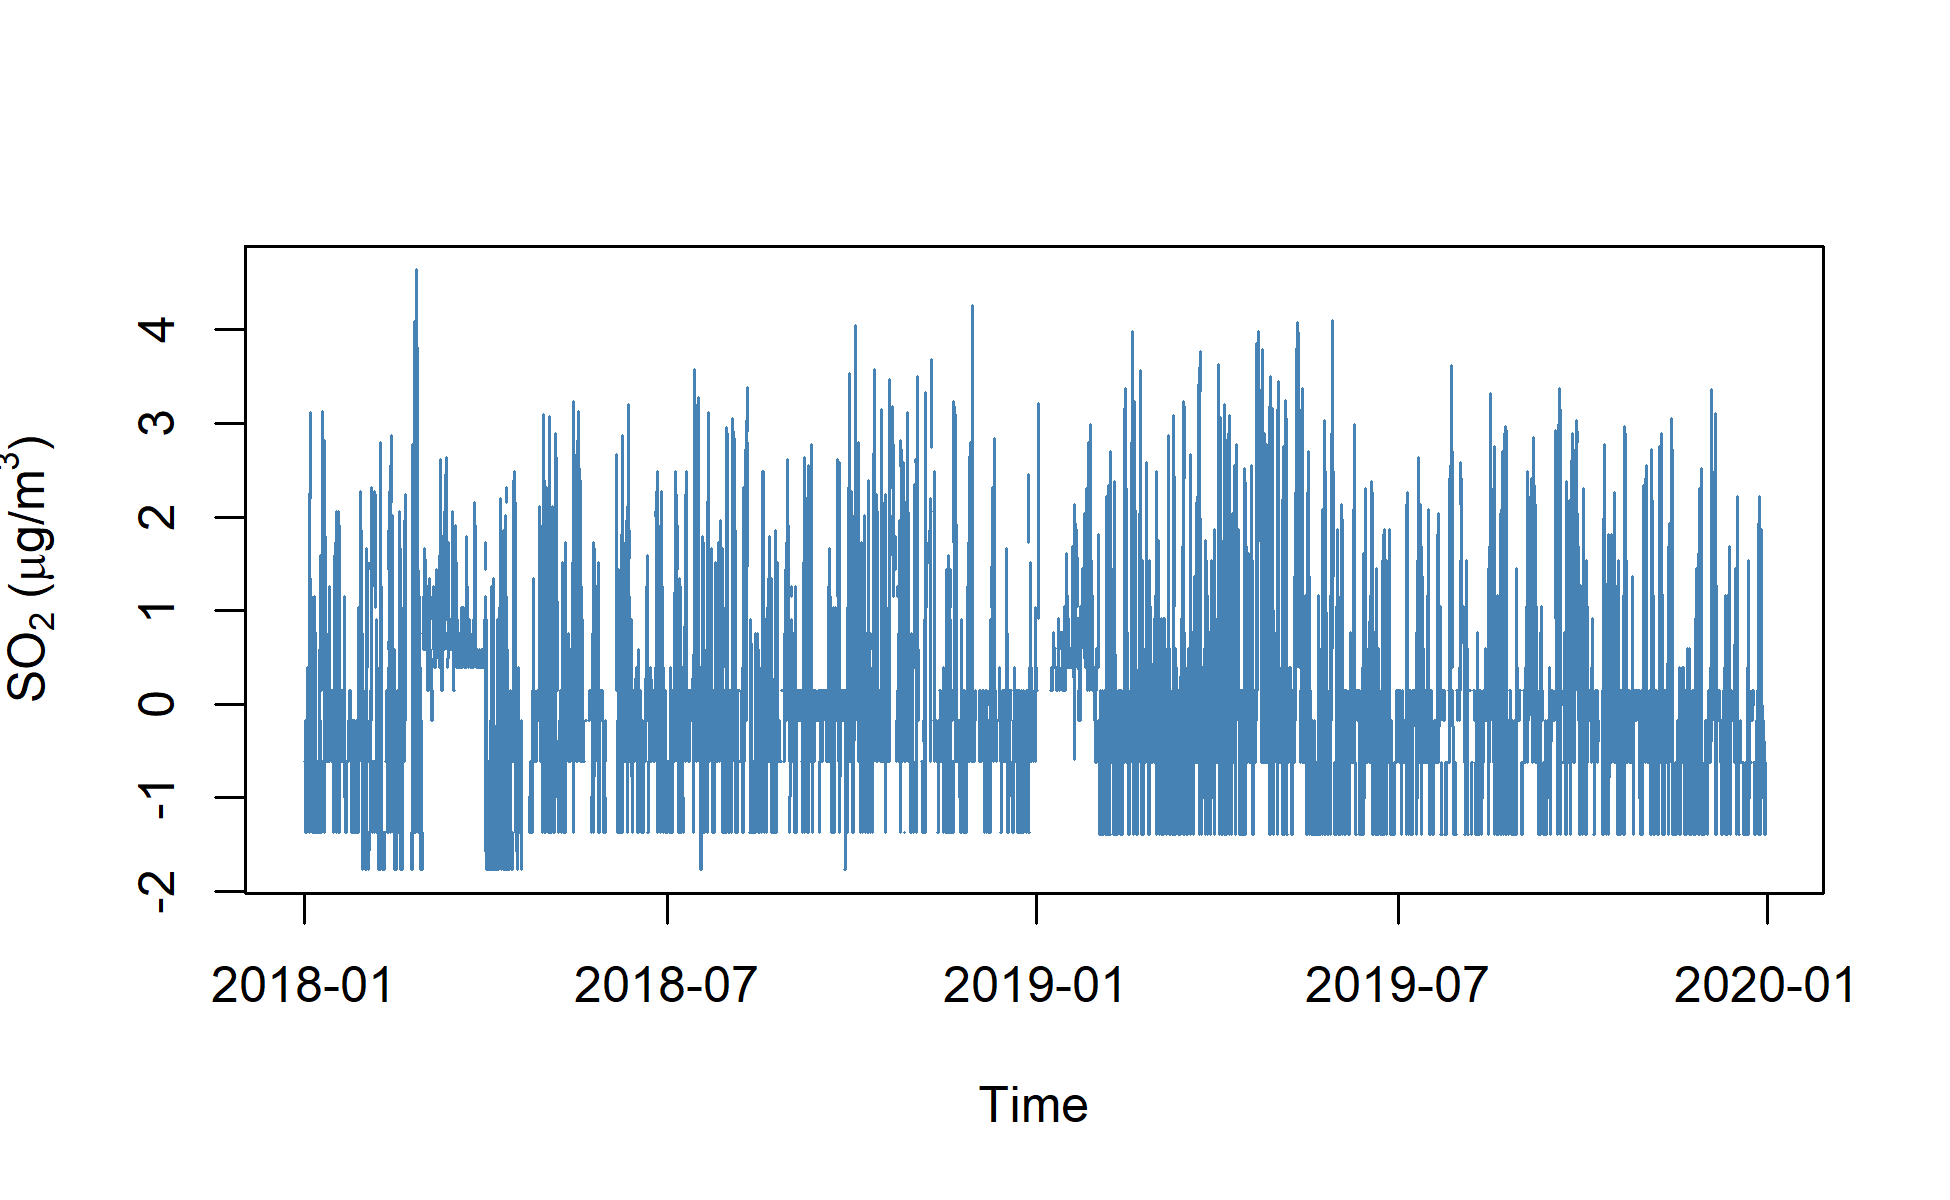
\includegraphics[width=\linewidth]{../img/transformed_so2.png}
         \caption{Sulphur dioxide}
         \end{subfigure}
         \hfill
         \begin{subfigure}{0.48\linewidth}
            \centering
            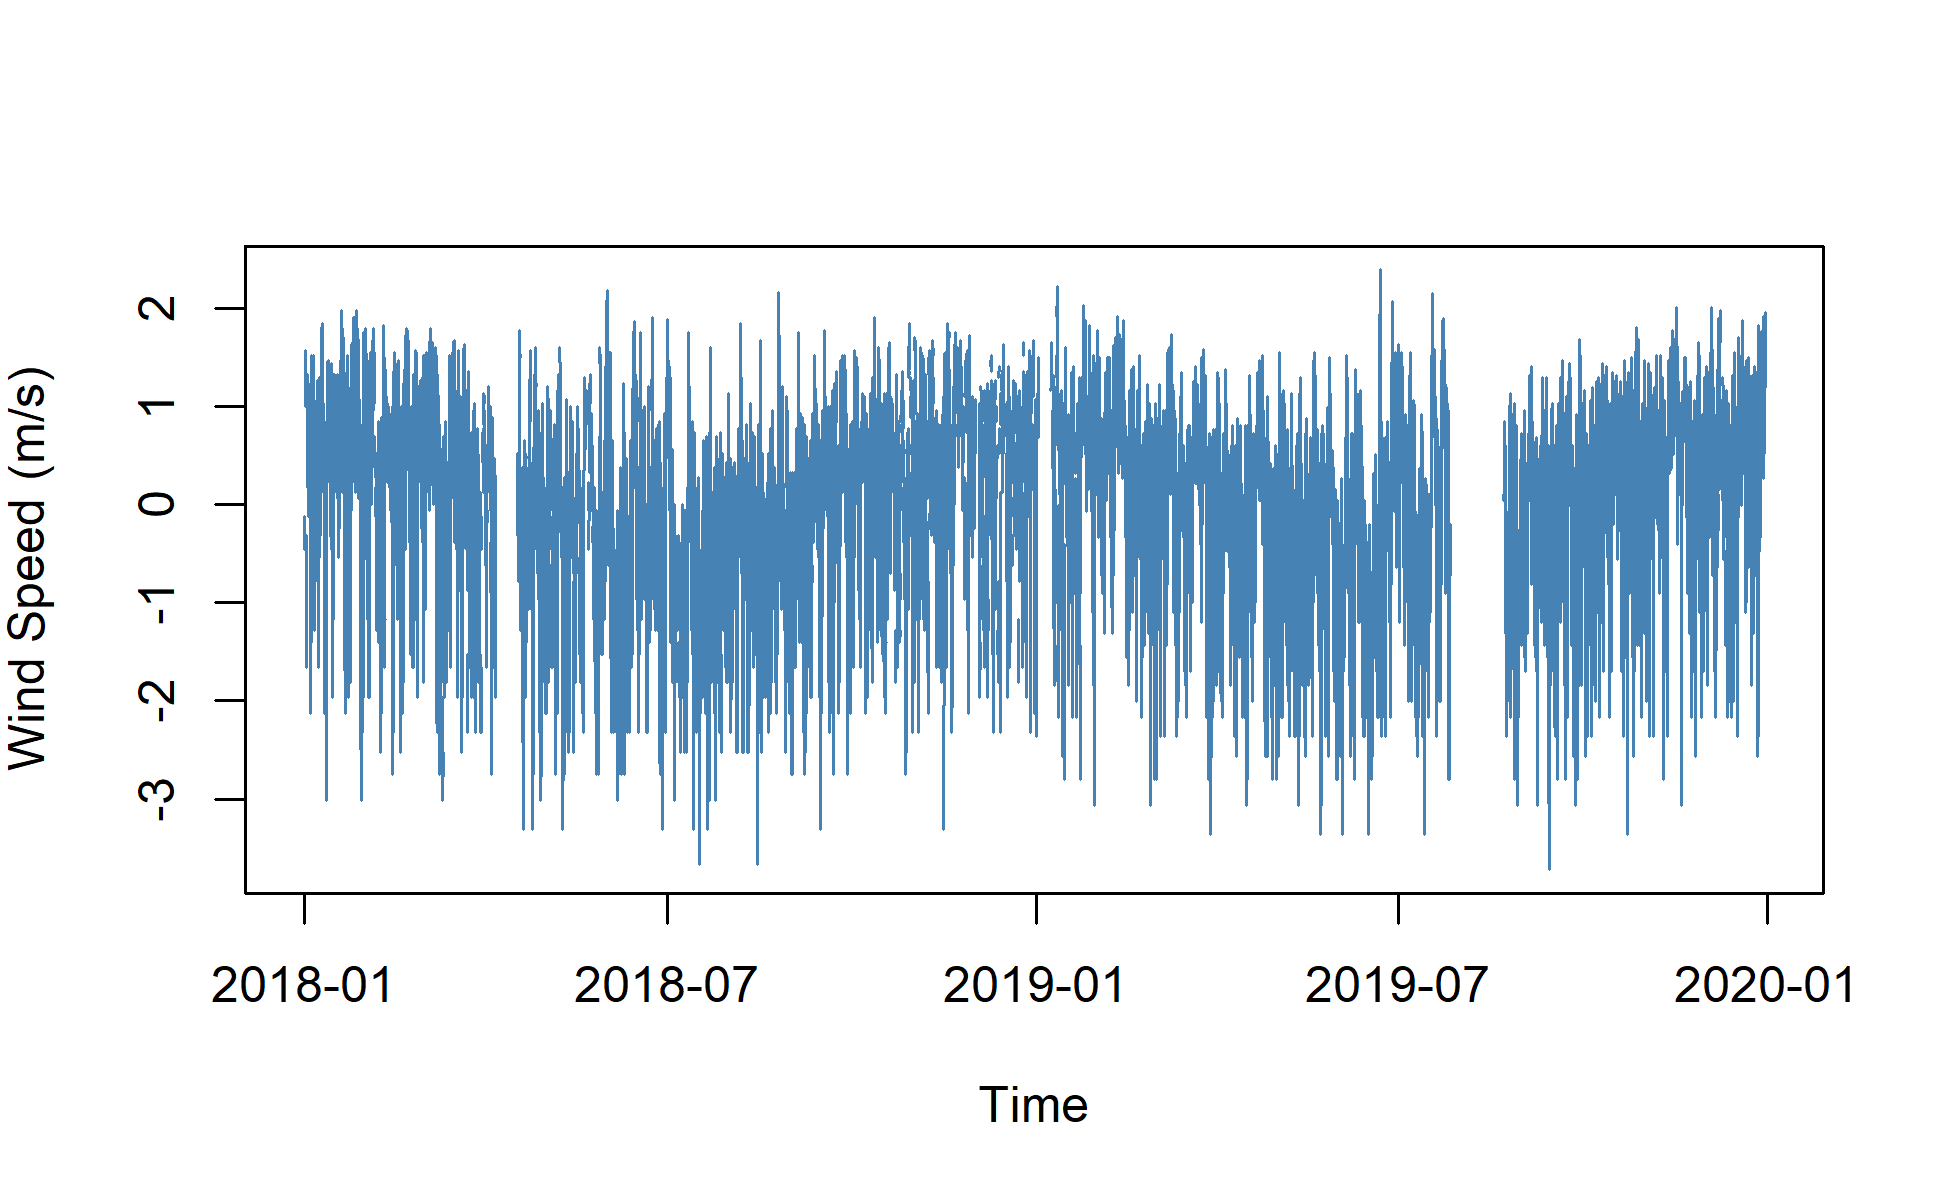
\includegraphics[width=\linewidth]{../img/transformed_speed.png}
            \caption{Wind speed}
         \end{subfigure}

         \caption{\textit{Post-processed daily curves of the nitrogen dioxide and meteorological data, both standardized by their overall mean and standard deviation.}}
      \end{figure}

      \subsection*{Components of the time series}     

      The response variable time-series $x_{t}$ is not statationary because the mean and variance are changing with time. To achieve stationarity there is a need for detrending and a variance stabilizing transformation. In order to stabilize the variance we use Box-Cox transformations in the training set, $y_{t} = (x_{t}^{\lambda} - 1) / \lambda$. The Box-Cox transformations allow us to experiment with a wide variety of $\lambda$ values. A good value of $\lambda$ is one the makes the variation in the data constant through time (Neil Watson, 2024). The \texttt{R} package \texttt{forecast} was used to perform the Box-Cox transformation which yielded an optimal value of $\hat{\lambda} \approx 0$, suggesting a logarithmic transformation. Then, conducting first-order differencing at lag one to remove the trend $z_{t} = y_{t} - y_{t-1} \, \text{for} \, t \in \{2, \, 3, \, \ldots, \, p\}$. The time series $z_{t}$ is now stationary. Thus, we only need to account for the mean and variance in our models.      

      \begin{figure}[H]
         \centering
         \begin{subfigure}{0.48\linewidth}
            \centering
            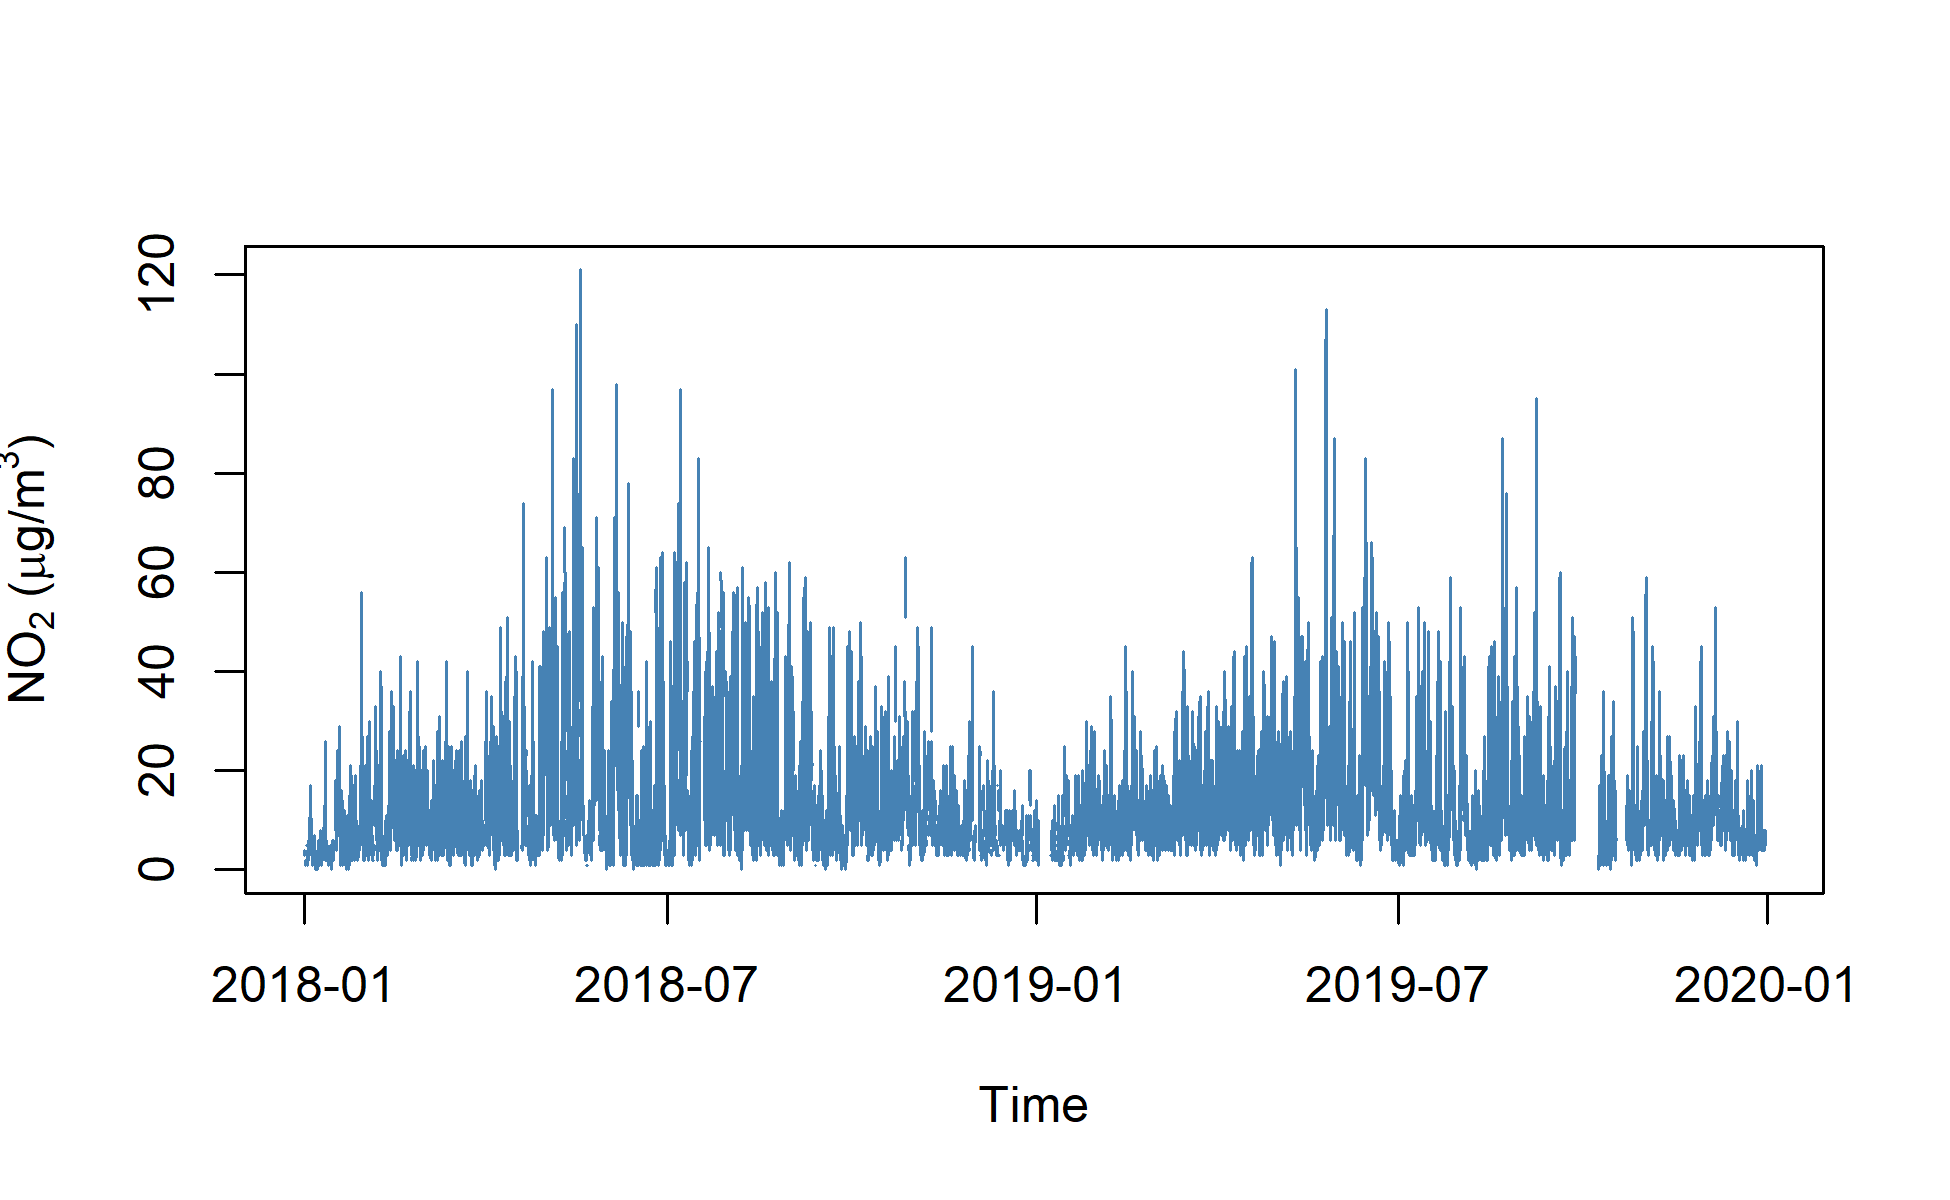
\includegraphics[width=\linewidth]{../img/extracted_no2.png}
            \caption{Before transformations.}
         \end{subfigure}
         \hfill
         \begin{subfigure}{0.48\linewidth}
            \centering
            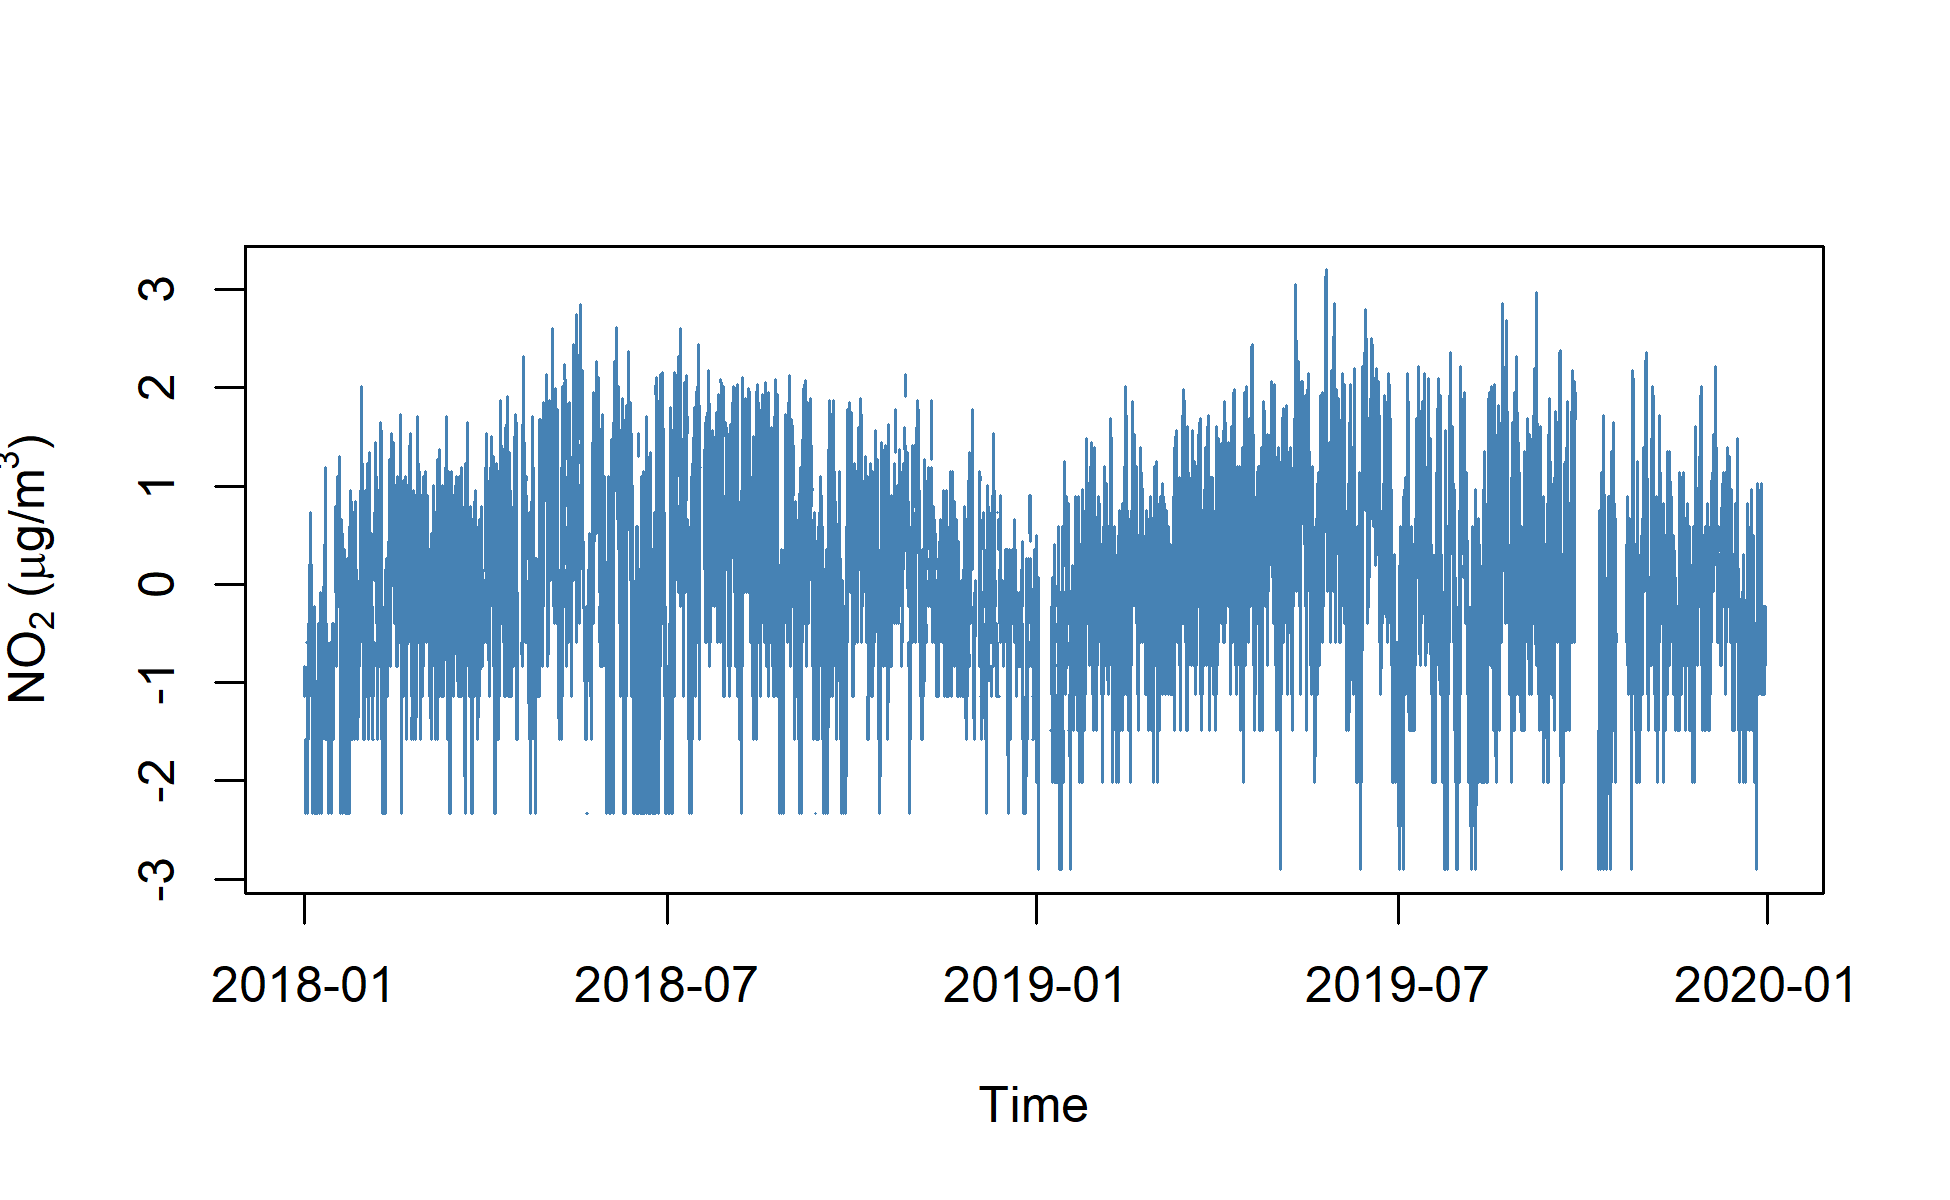
\includegraphics[width=\linewidth]{../img/transformed_no2.png}
            \caption{After transformations.}
         \end{subfigure}
         \caption{\textit{Comparison of NO\textsubscript{2} time series before and after transformations.}}
      \end{figure}

      \subsection*{Results}

      \begin{table}[H]
         \centering
         \begin{tabular}{lcccccc}
         \hline
         \multirow{2}{*}{Model} & \multicolumn{3}{c}{RMSE} & \multicolumn{3}{c}{MAE} \\
         \cline{2-7}
         & \multicolumn{3}{c}{Forecasts} & \multicolumn{3}{c}{Forecasts} \\
         & \multicolumn{3}{c}{($h$ day time horizon)} & \multicolumn{3}{c}{($h$ day time horizon)} \\
         & 24 & 168 & 720 & 24 & 168 & 720 \\
         \hline
         Average & 8.61 & 7.16 & 6.62 & 8.54 & 6.48 & 5.73 \\
         \rowcolor{blue!20} Naive & 1.35 & 5.58 & 7.10 & 1.00 & 3.59 & 4.80 \\
         SNaive & 3.72 & 5.71 & 7.21 & 2.48 & 4.05 & 5.28 \\
         Drift & 1.35 & 5.59 & 7.16 & 1.00 & 3.60 & 4.86 \\
         ARIMA & 5.01 & 6.46 & 6.45 & 4.91 & 5.81 & 5.57 \\
         \rowcolor{red!20} GP & 6.07 & 8.73 & 10.72 & 5.47 & 7.29 & 9.14 \\
         \hline
         \end{tabular}
         \caption{\textit{RMSE and MAE of forecasting models across horizons.}}
      \end{table}

   \section*{References}
      \begin{enumerate}
         \item https://www.lung.org/clean-air/outdoors/what-makes-air-unhealthy/nitrogen-dioxide
      \end{enumerate}
   
   \end{flushleft}
\end{document}
